%%%%%%%%%%%%%%%%%%%%%%%%%%%%%%%%%%%%%%%%%%%%%%%%%%%%%%%%%%%%%%%
%
% Welcome to Overleaf --- just edit your LaTeX on the left,
% and we'll compile it for you on the right. If you open the
% 'Share' menu, you can invite other users to edit at the same
% time. See www.overleaf.com/learn for more info. Enjoy!
%
%%%%%%%%%%%%%%%%%%%%%%%%%%%%%%%%%%%%%%%%%%%%%%%%%%%%%%%%%%%%%%%


% Inbuilt themes in beamer
\documentclass{beamer}
\usepackage[utf8]{inputenc}
\usepackage{amsmath}
\usepackage{amsfonts}
\usepackage{mathtools}
\usepackage{amssymb}
\providecommand{\pr}[1]{\ensuremath{\Pr\left(#1\right)}}


% Theme choice:
\usetheme{CambridgeUS}

% Title page details: 
\title{AI1110 Assignment-8} 
\author{Gollapudi Sasank CS21BTECH11019}
\date{\today}
\logo{\large \LaTeX{}}


\begin{document}

% Title page frame
\begin{frame}
    \titlepage 
\end{frame}

% Remove logo from the next slides
\logo{}


% Outline frame
\begin{frame}{Outline}
    \tableofcontents
\end{frame}


% Lists frame
\section{Question}
\begin{frame}{Question}
A fair coin is tossed twice , and let the random variable $X$ represent the number of heads. Find $F_X(x)$ (Cummulative Distribution Function of X) 
\end{frame}


% Blocks frame
\section{Solution}
\begin{frame}{Solution}
Let us denote Head by $H$ and tail by $T$. \\
Sample Space(S) = \{HH,HT,TH,TT\}.\\
$X$ : Number of heads obtained
\begin{align}
X(HH) = 2 \\
X(HT) = 1 \\
X(TH) = 1 \\
X(TT) = 0 
\end{align}
\begin{align}
\pr{X=0} = \frac{1}{4} \\
\pr{X=1} = \frac{1}{2} \\
\pr{X=2} = \frac{1}{4}
\end{align}
\end{frame} 

\begin{frame}
From the definition of Cummulative Distribution Function(CDF) of a random variable $X$ 
\begin{align}
F_X(x) = \pr{X \le x}
\end{align}
For $x<0 $ , $X \le x \Rightarrow X<0$
\begin{align}
F_X(x) &= \pr{X<0} \\
F_X(x) &= 0
\end{align}
For $0 \le x < 1 $ , $X \le x \Rightarrow X<1$
\begin{align}
F_X(x) &= \pr{X < 1} \\
F_X(x) &= \pr{X=0} \\
F_X(x) &= \frac{1}{4}
\end{align}
\end{frame}
\begin{frame}
For $ 1 \le x < 2$ , $X \le x \Rightarrow X<2$
\begin{align}
F_X(x) &= \pr{X < 2} \\
F_X(x) &= \pr{X=0} + \pr{X=1}  \\
F_X(x) &= \frac{1}{4} + \frac{1}{2} \\
F_X(x) &= \frac{3}{4}  
\end{align}
For $ x \ge 2 $ , $X \le x \Rightarrow X<\infty$
\begin{align}
F_X(x) &= \pr{X=0} + \pr{X=1} + \pr{X=2} \\
F_X(x) &= \frac{1}{4} + \frac{1}{2} + \frac{1}{4} \\
F_X(x) &= 1
\end{align}
\end{frame}
\section{Graph}
\begin{frame}{Graph}
\begin{figure}[h]
\centering
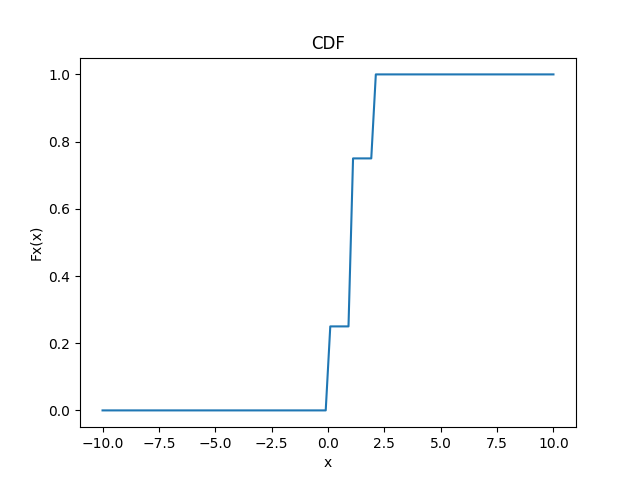
\includegraphics[width=0.7\columnwidth]{Fig1.png}
\caption{CDF graph}
\label{Fig 1}
\end{figure}
\end{frame}
\end{document}